\setlength{\footskip}{8mm}

\chapter{Literature Review} 
\label{ch:literature-review}

\textit{Some intro..}

\section{Section Name in Literature Review}
\label{section-name-in-literature-review}

Example text below ..

apply the background subtraction 
technique to extract blobs or human from a scene by the 
following conditions:
\[
\begin{array}{lc}
  {\rm if} & \left|{I_a (x,y) - I_b (x,y)}\right|< T,\;I_e (x,y) = 0 \\ 
  {\rm else} & I_e (x,y) = I_a (x,y), 
\end{array}
\]
where $I_e (x,y)$ is a human extracted image, $I_a (x,y)$ is an
original image, $I_b (x,y)$ is a background image, and $T$ is a
threshold. Figure~\ref{fig:mesh-feature} shows something. Some work also uses 
mesh features~.

% THE REASON ~ IS USED HERE BECAUSE WE TELL LATEX THAT THESE TWO WORDS SHOULD 
% GO TOGETHER IN THE SAME LINE.

\begin{figure}[t]
  \centering
  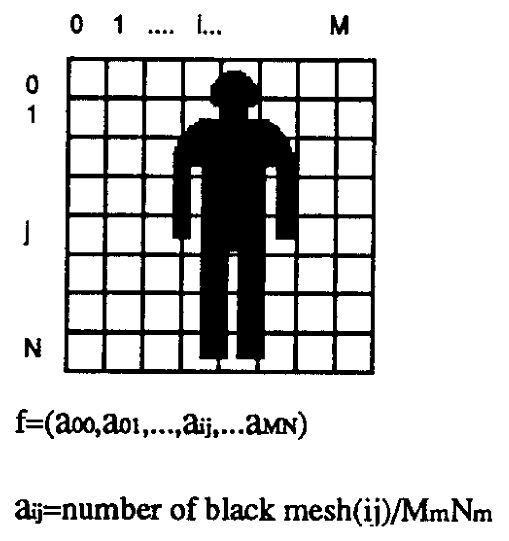
\includegraphics[width=2in]{figures/mesh-feature.jpg}  
  \caption[Mesh feature calculation]{Mesh feature
    calculation. Reprinted from the work of Yamato et al.\ (1992).}
  \label{fig:mesh-feature}
\end{figure}

\FloatBarrier

